% This is a comment. It is a comment because the line begins with a '%'. That means that LaTex does not read this when it compiles. I can write WHATEVER I want to myself and no one else will ever see it if I only show them the PDF of my paper!

% First you need to declare the document type. We will write an 'article.' The other typical options are 'letter' or 'report' or 'beamer' which creates powerpoints.
\documentclass{article}

%------------PACKAGES--------------------------------
% This is where you import LaTex packages (at the very top, below the document class). Packages expand the capabilities of LaTex. You can download them from the internet to do things like create graphs, include pictures, change fonts, or even include a picture of the Simpsons.

% Let's import the ams math package so that we can use LaTex math mode. Importing the package looks like:
\usepackage{amsmath}
\usepackage{amsthm}
\usepackage{graphicx}

%---------BEGIN---------------------------------------
% In order for tex to compile, you need to tell it to begin and end the document. This is done by typing '\begin{document},' which is already done below:
\begin{document}

% Task 1: Go to the very bottom of this and type '\end{document}. Then compile and see how it looks so far. If you are using TexMaker, you can do so by clicking the arrow to the left of the 'QuickBuild' button in the top toolbar.


% We're going to have a LaTex adventure! Put your name, your quest, and your favorite color at the top so that everyone knows whose adventure it is.
% Your prof needs you to put your name on the top RIGHT hand side of the page. This can be done by using the pair of  commands '\begin{flushright}' and '\end{flushright}'.
% Task 2: Change the info between the flush right commands to your own name, quest, favorite color.
\begin{flushright}
Professor Fishy McMittens\\
I want to learn to LaTex like a superhero.\\
My fave color is def purple.
\end{flushright}

% Task 3: Compile and see what happens. You should compile often so when there are mistakes they can be fixed as soon as they are made.

% Oh no! If you've never used Tex before, most likely your name, quest, and favorite color were all printed on one line, even if you hit 'enter' between the three. 
% This happens because LaTex is NOT a 'What You See is What You Get' word processor the way Microsoft Word is. You need to TELL tex that you want line breaks between your lines. It uses the line break command '\\' (without quotes).

% Task 4: The line break command is '\\'. Go back up and put line breaks between your name, quest, and fave color. Compile again to see if it worked.

% Now we're on to the body of the document. I needed a writing prompt, so I looked some up online. One is 'Where would you go if you could teleport to any one place for free for 24 hours? Nothing is out: the moon or the bottom of the ocean are both options.' So we will go with that. 

% Task 5: Write a sentence saying where you will go.

I want to teleport to Budapest.

% I need you to prove it to me! In order to format proofs in Tex, we need to import the amstheorems package.

% Task 6: Return to the top where we imported packages and type '\usepackage{amsthm}'

% Task 7: Write a two paragraph 'Proof' about why you are choosing to go there. Use the pair of commands '\begin{proof}' and '\end{proof}'. Separate your paragraphs by typing '\par' after the first one and before the second one.

\begin{proof}
Budapest is great because it is actually two cities: Buda and Pest (well, it used to be anyway).
\par It is also great because you can use the slogan 'Pest City Ever' if you both (a), live on the Pest side and (b), speak English better than Hungarian.
\end{proof}

% Let's put in a picture of this place or something unique about this place. We need to add another package first.

% Task 8: Add the package '\usepackage{graphicx}'

% Task 9: Choose a picture from the internet. Download it and save it in the same folder that this tex document is saved in. 


%Task 10: Uncomment the command below. Change 'picturename.png' to the name of your photo that is now saved in the folder. You can get rid of the '.jpg' or '.png' 
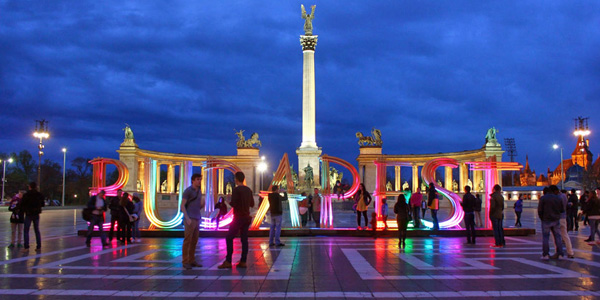
\includegraphics[width=.5\linewidth]{budapest-web3}

% Lets add some math. We already imported the package that lets us use math mode, which is denoted on both sides of the math by the dollar sign '$'. If you want to center the math, use two dollar signs on each side. For example:
\par Some math is: $5 + 5 = 10$ or $1^0 = 1$ or $\frac{1}{2} - \frac{1}{2} = 0$.
\par I like to type math in this Budapest. Some more math is:

% Some important symbols and their commands can be found at this site: http://web.ift.uib.no/Teori/KURS/WRK/TeX/symALL.html
% Note that there are some commands which can ONLY be used in math mode, and some which can ONLY be used outside of math mode. For example, '\par' can only be used outside of math mode, and '\frac{•}{•}' can only be used in math mode. The line break '\\' can be used in both.

% Task 11: Type two lines of math below, using line breaks in between.
$4 \times 4 = 16$\\
$11 + 1 = 12$\\

% Task 12: Type another line of math below, this time using TWO dollar signs on each side of the math line. Compile and check out what happened.
$$4 + 4 = 8$$\\

% One more thing about math mode: what if you want to actually USE the dollar sign in math mode? Then you just precede it with a forwardslash. Use '\$' to get an actual dollar sign. The same thing goes for a set bracket: '\{' or '\}'.

% What do you want to do on this adventure? Let's make a list. 
% Task 13: List three things you want to do in this place. Uncomment the following five lines and replace the A,B,C with your three things you want to do in this place.
I want to:
\begin{itemize}
\item Go to Szechenyi Bath.
\item Ride the Sziget Eye.
\item Drink 'Csak Jo Sor.' :)
\end{itemize}

% And what are the BEST three things about this place? List them in order! Use the pair of commands '\begin{enumerate} and '\end{enumerate}' this time in place of 'itemize'. Use the commad '\item' in the same way as we did with itemize to separate the bullet points.
Three of the BEST things about this place are:
% Task 14: Make a list of three things about the place using the enumerate command.
\begin{enumerate}
\item Public transit.
\begin{enumerate}
\item Buses + Trams + Metro
\item The YELLOW LINE is so old and wonderful.
\end{enumerate}
\item 'Wet air', not rain
\item Tall ceilings.
\end{enumerate}

% Can we make lists of lists? Of Course!
% Task 15: Go back to the list you just made. Use the  '\begin{enumerate} and '\end{enumerate}' commands again, this time between the first and second item. Create a sublist of two reasons the best thing about the place is the best thing about the place.

% Lets finish this mini paper with one more line about the trip. 

% Task 16: Write one more sentence which sums up the place you chose to travel to. Center it by writing the line in between commands '\begin{center}' and '\end{center}'.
\begin{center}
I loved my time in Bp and would love to teleport back just for a day.
\end{center}

\end{document}